\subsubsection{Densidad de aportes}

La densidad promedio de aportes es calculada como el cociente entre la
cantidad total de activos que durante el año han aportado exactamente 1,
2, 3\ldots{}, 12 meses y el número de meses potencialmente aportados por
el total de asegurados, es decir una rela ción entre los aportes reales
y los potenciales.

Una mirada al Gráfico xx destaca que prácticamente no existen
diferencias por sexo entre el número de meses cotizados a lo largo del
periodo considerado, y se observa que alrededor del xx\% de hombres y
mujeres realizaron aportes los 12 meses del año 20 20.

El Gráfico xx evidencia que el número promedio de meses cotizados es
bajo para los tramos de edades más jóvenes, lo que podría explicarse por
una alta movilidad laboral, dedicación de tiempo parcial a los estudios
y/o informalidad laboral. En tanto aum enta la edad, el promedio del
número de meses de aportes también aumenta. Por otra parte, no se
aprecian diferencias por sexo en las edades inferiores a los 35 años. A
partir de dicha edad si se observa que existe un comportamiento
favorable para las m ujeres, en el sentido que, a medida que aumenta la
edad de las mujeres se incrementa el número promedio de meses cotizados
en el año.

\begin{table}[H]
\begin{center}
\footnotesize
\caption{\bf{Cantidad de cotizantes por la densidad de cotizaciones, según sexo}}
\begin{tabular}{l|rrrrrrrrrrr}
 & \multicolumn{6}{c}{\textbf{Sexo}} \\
\textbf{Densidad de cotizaciones (tramos)} & \multicolumn{2}{c}{\textbf{Hombres}} & \multicolumn{2}{c}{\textbf{Mujeres}} & \multicolumn{2}{c}{\textbf{Total}} \\
\hline
0 a 10\%&195.074&20,2943\%&105.347&19,1556\%&300.421&19,8799\% \\
11 a 19\%&113.505&11,8084\%&61.939&11,2626\%&175.444&11,6097\% \\
20 a 29\%&85.756&8,9215\%&47.615&8,6580\%&133.371&8,8256\% \\
30 a 39\%&67.369&7,0087\%&37.099&6,7458\%&104.468&6,9130\% \\
40 a 49\%&59.557&6,1959\%&32.900&5,9823\%&92.457&6,1182\% \\
50 a 59\%&61.792&6,4285\%&34.019&6,1858\%&95.811&6,3401\% \\
60 a 69\%&55.312&5,7543\%&31.534&5,7339\%&86.846&5,7469\% \\
70 a 79\%&54.536&5,6736\%&30.658&5,5746\%&85.194&5,6376\% \\
80 a 89\%&64.363&6,6959\%&38.704&7,0377\%&103.067&6,8203\% \\
90 a 99\%&117.156&12,1882\%&81.050&14,7376\%&198.206&13,1160\% \\
100\%&86.805&9,0307\%&49.089&8,9260\%&135.894&8,9926\% \\
\textbf{Total}&961.225&100,0000\%&549.954&100,0000\%&1.511.179&100,0000\% \\

\end{tabular}
                    \item \footnotesize Fuente : Elaboración própia a partir de registros administrativos del IPS.
                    \item \footnotesize Nota : 
\end{center}
\end{table}

\begin{figure}[H]
\begin{center}
                    \caption{Densidad de cotizaciones}
                    \vspace{0.5cm}
                    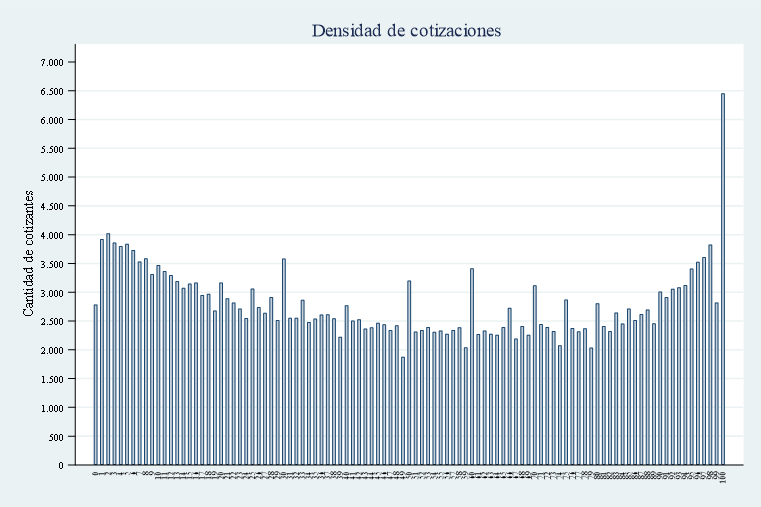
\includegraphics[scale=0.35]{dencot.png}
\end{center}
\end{figure}

\begin{figure}[H]
\begin{center}
                    \caption{Densidad de cotizaciones}
                    \vspace{0.5cm}
                    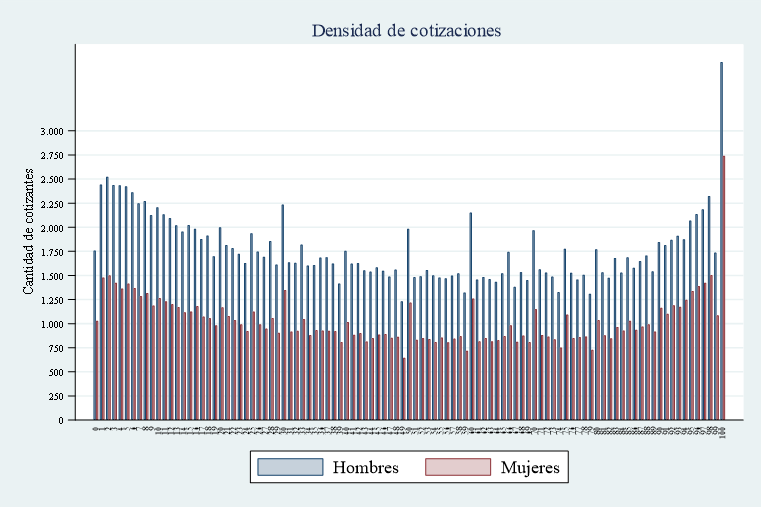
\includegraphics[scale=0.35]{dencot_by_sex}
\end{center}
\end{figure}
